\documentclass[aspectratio=169,11pt]{beamer}

\usetheme{Frankfurt}
\usecolortheme{default}

\usepackage[T1]{fontenc}
\usepackage[utf8]{inputenc}
\usepackage[polish]{babel}
\usepackage{amsmath}
\usepackage{amssymb}
\usepackage{graphicx}
\usepackage{booktabs}
\usepackage{listings}
\usepackage{tikz}
\usetikzlibrary{positioning,arrows.meta,shapes.geometric}

\setbeamertemplate{navigation symbols}{}
\setbeamertemplate{bibliography item}[text]

\setbeamertemplate{footline}{
  \leavevmode%
  \hbox{%
    \begin{beamercolorbox}[wd=.333333\paperwidth,ht=2.25ex,dp=1ex,center]{author in head/foot}%
      \usebeamerfont{author in head/foot}\insertshortauthor
    \end{beamercolorbox}%
    \begin{beamercolorbox}[wd=.333333\paperwidth,ht=2.25ex,dp=1ex,center]{title in head/foot}%
      \usebeamerfont{title in head/foot}\insertshorttitle
    \end{beamercolorbox}%
    \begin{beamercolorbox}[wd=.333333\paperwidth,ht=2.25ex,dp=1ex,right]{date in head/foot}%
      \usebeamerfont{date in head/foot}\insertframenumber{} / \inserttotalframenumber\hspace*{2ex}
    \end{beamercolorbox}}%
  \vskip0pt%
}

\lstset{
  basicstyle=\ttfamily\scriptsize,
  frame=single,
  breaklines=true,
  columns=fullflexible,
  keepspaces=true,
  showstringspaces=false
}

\newcommand{\authorone}{Bartosz Jardzioch}
\newcommand{\authortwo}{Maciej Jarząbek}
\newcommand{\authorthree}{Filip Hendryk}

\title[Wpływ kompresji obrazu na OCR]{Wpływ kompresji obrazu na skuteczność systemów optycznego rozpoznawania znaków (OCR)}
\subtitle{Zespołowy projekt badawczy}
\author[\authorone, \authortwo, \authorthree]{\authorone \and \authortwo \and \authorthree}
\date{}

\begin{document}

\begin{frame}
  \titlepage
\end{frame}

\begin{frame}{Plan prezentacji}
  \tableofcontents
\end{frame}

\section{Wprowadzenie}

\begin{frame}{Cel projektu}
  \begin{itemize}
    \item Oceniamy, jak pogorszenie jakości obrazu wpływa na skuteczność OCR
    \item Porównujemy trzy popularne systemy OCR w jednakowych warunkach
  \end{itemize}
  \vspace{0.5em}
  \begin{block}{Pytanie badawcze}
    Jak kompresja, zmniejszenie rozdzielczości i szum wpływają na jakość rozpoznawanego tekstu?
  \end{block}
\end{frame}

\begin{frame}{Przegląd literatury}
  \footnotesize
  \setlength{\itemsep}{0.2em}
  \begin{itemize}
    \item Optical character recognition based document image quality assessment~\cite{frsip2026}
    \item TrOCR: Transformer-Based Optical Character Recognition with Pre-trained Models~\cite{trocr2021}
    \item PaddleOCR 3.0 Technical Report~\cite{paddleocr2025}
    \item Calamari -- A High-Performance Tensorflow-based Deep Learning Package for Optical Character Recognition~\cite{calamari2020}
    \item When Good OCR Is Not Enough: Benchmarking OCR Robustness for Retrieval-Augmented Generation~\cite{ragocr2026}
    \item Enhancing OCR Accuracy with Super Resolution~\cite{superres2018}
    \item Open-Source Document-Image Compression and OCR Degradation: A Reproducible, Multi-Axis Evaluation~\cite{compression2026}
    \item Assessing the Impact of Image Resolution on OCR Transcription Accuracy~\cite{resolution}
    \item Optical Character Recognition of 19th Century Classical Commentaries: the Current State of Affairs~\cite{commentaries2021}
    \item Image Preprocessing for Improving OCR Accuracy~\cite{preprocessing2007}
  \end{itemize}
\end{frame}

\begin{frame}{Testowane systemy OCR}
  \begin{columns}[T]
    \begin{column}{0.32\textwidth}
      \begin{block}{Tesseract}
        Podejście hybrydowe\\
      \end{block}
    \end{column}
    \begin{column}{0.32\textwidth}
      \begin{block}{EasyOCR}
        Głębokie sieci neuronowe\\
      \end{block}
    \end{column}
    \begin{column}{0.32\textwidth}
      \begin{block}{PaddleOCR}
        Głębokie sieci neuronowe\\
      \end{block}
    \end{column}
  \end{columns}
\end{frame}

\section{Zbiór danych}

\begin{frame}{Zbiór danych: FUNSD}
  \begin{columns}[T]
    \begin{column}{0.5\textwidth}
      \textbf{Form Understanding in Noisy Scanned Documents}~\cite{jaume2019}
      \begin{itemize}
        \item Skany formularzy z ręcznymi i drukowanymi wypełnieniami
        \item Dokumenty niskiej jakości
        \item Typy dokumentów: formularze, ankiety, raporty, pisma urzędowe
      \end{itemize}
    \end{column}
    \begin{column}{0.5\textwidth}
      \centering
      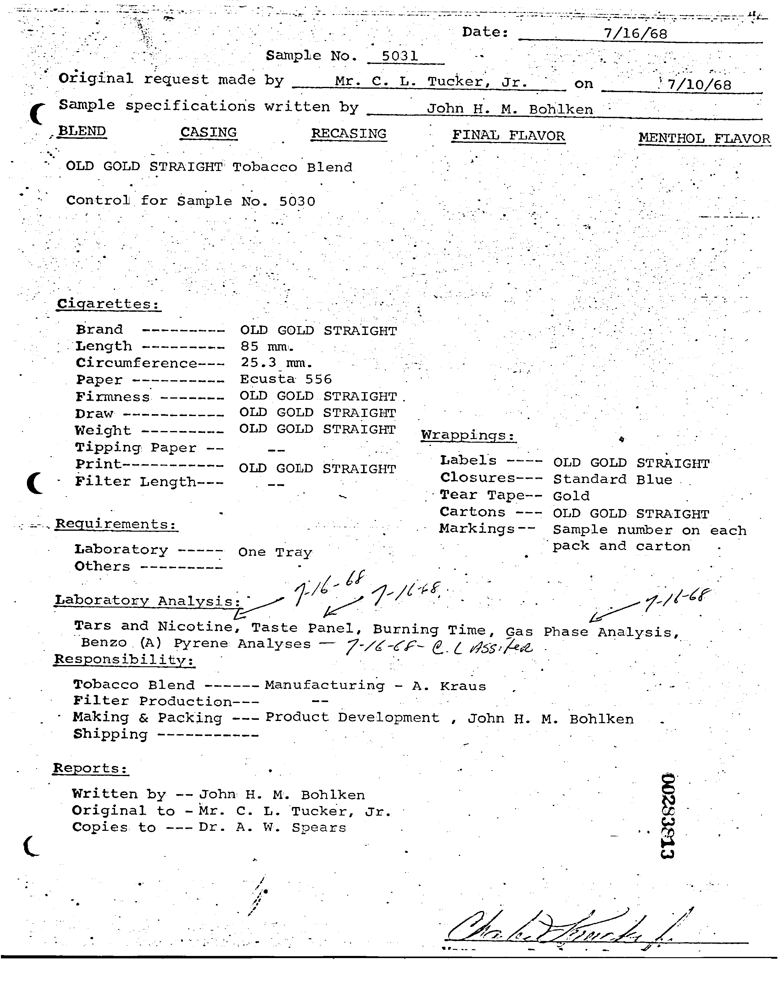
\includegraphics[height=0.82\textheight,width=\textwidth,keepaspectratio]{form.png}
    \end{column}
  \end{columns}
\end{frame}

\begin{frame}[fragile]{Etykiety w zbiorze FUNSD}
  \begin{columns}[T]
    \begin{column}{0.5\textwidth}
      \begin{itemize}
        \item Ramki otaczające fragmenty tekstu (\emph{bounding boxes})
        \item Tekst referencyjny (\emph{ground truth}) dla każdej ramki
        \item Podział na słowa oraz typy elementów: pytanie, odpowiedź, nagłówek
      \end{itemize}
      \vspace{0.5em}
      \begin{alertblock}{Zastosowanie w testach}
        Etykiety pozwalają automatycznie obliczać metryki jakości OCR.
      \end{alertblock}
    \end{column}
    \begin{column}{0.5\textwidth}
\begin{lstlisting}
{
  "box": [96, 141, 141, 158],
  "text": "FROM:",
  "label": "question",
  "words": [
    {
      "box": [96, 141, 141, 158],
      "text": "FROM:"
    }
  ],
  "linking": [],
  "id": 1
}
\end{lstlisting}
    \end{column}
  \end{columns}
\end{frame}

\begin{frame}{Statystyki wczytanych obrazów}
  \begin{center}
    \begin{tabular}{lc}
      \toprule
      Statystyka & Wartość \\
      \midrule
      Liczba obrazów w zbiorze& 149\\
      Liczba zaszumionych & 447\\
      Liczba przeskalowanych & 596\\
      Liczba skompresowanych & 447\\
      Liczba ramek z tekstem & 7411\\
      \bottomrule
    \end{tabular}
  \end{center}
\end{frame}

\section{Metodyka}

\begin{frame}{Metody pogarszania jakości obrazu}
  \begin{columns}[T]
    \begin{column}{0.32\textwidth}
      \begin{block}{Kompresja JPEG}
        Stopień kompresji
      \end{block}
    \end{column}
    \begin{column}{0.32\textwidth}
      \begin{block}{Skalowanie}
        Współczynnik zmiany rozdzielczości
      \end{block}
    \end{column}
    \begin{column}{0.32\textwidth}
      \begin{block}{Zaszumianie}
        Szum gaussowski o odchyleniu $\sigma$
      \end{block}
    \end{column}
  \end{columns}
  \vspace{0.8em}
\end{frame}

\begin{frame}{Proces badawczy}
  \centering
  \begin{tikzpicture}[
      node distance=0.6cm,
      box/.style={rectangle, rounded corners, draw=black, fill=blue!10, minimum height=1.2cm, text width=2.3cm, align=center, font=\small},
      arrow/.style={-{Stealth[length=2.5mm]}, thick}
    ]
    \node[box] (original) {Obraz ze zbioru};
    \node[box, right=of original] (degrade) {Pogorszenie jakości};
    \node[box, right=of degrade] (ocr) {OCR};
    \node[box, right=of ocr] (metrics) {Metryki jakości};
    \draw[arrow] (original) -- (degrade);
    \draw[arrow] (degrade) -- (ocr);
    \draw[arrow] (ocr) -- (metrics);
  \end{tikzpicture}
  \vspace{0.8em}
  \begin{itemize}
    \item Dla każdej operacji testujemy wiele wartości parametrów
    \item Porównujemy wyniki wszystkich systemów na tych samych obrazach
  \end{itemize}
\end{frame}

\begin{frame}{Przykładowe modyfikacje obrazu}
  \centering
  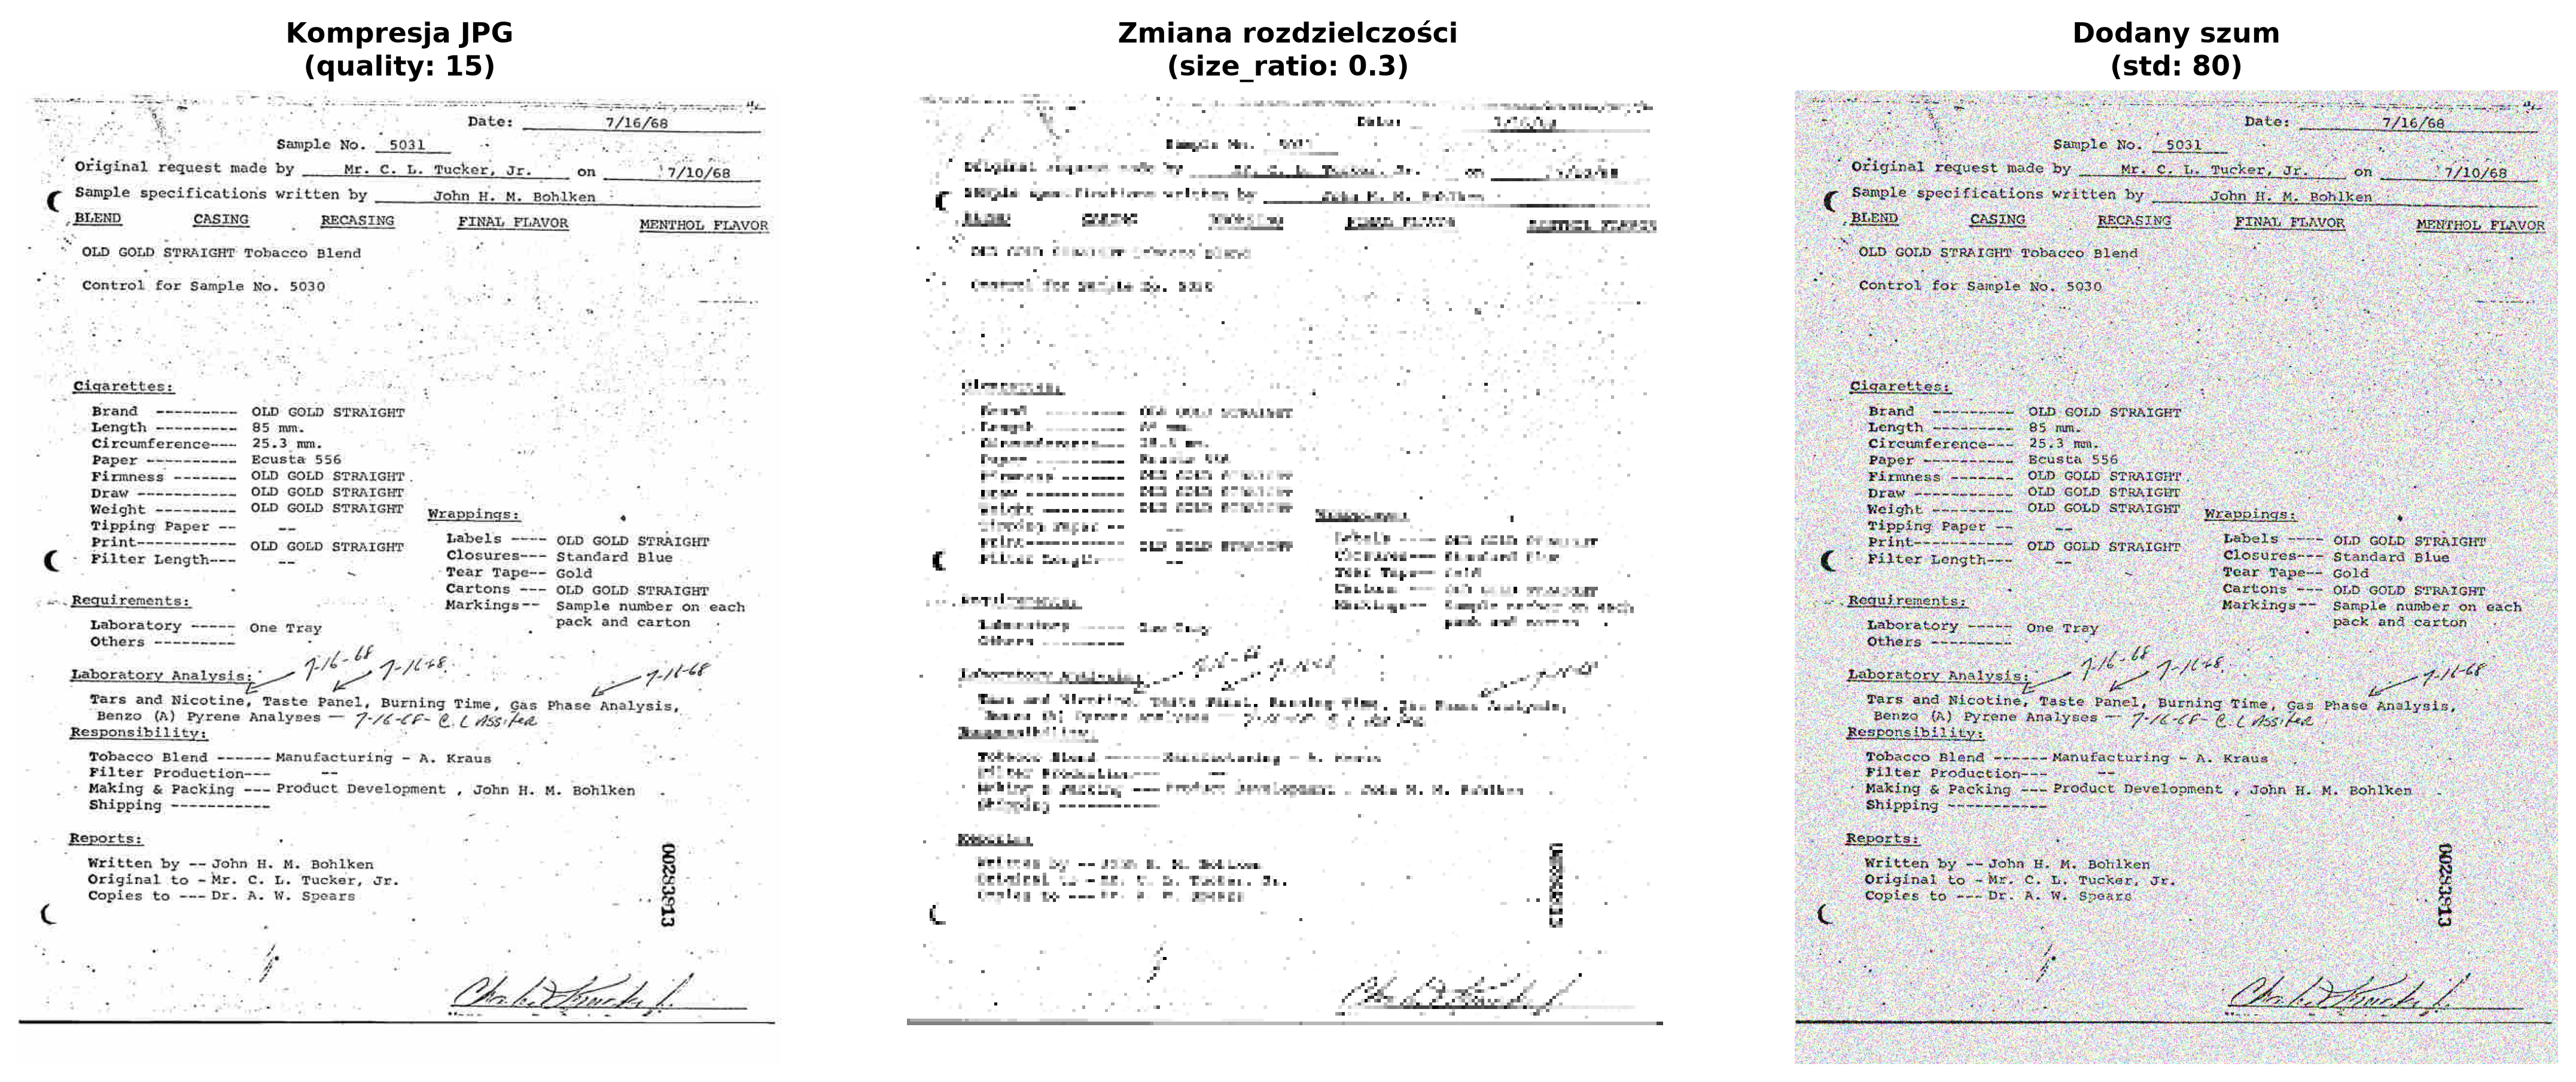
\includegraphics[width=\textwidth,height=0.75\textheight,keepaspectratio]{form_efekty.png}
\end{frame}

\begin{frame}{Metryki jakości}
  \begin{columns}[T]
    \begin{column}{0.58\textwidth}
      \small
      Porównujemy tekst rozpoznany przez OCR z tekstem referencyjnym:
      \begin{itemize}
        \item $S$ -- liczba znaków błędnie zastąpionych innymi znakami
        \item $D$ -- liczba znaków pominiętych przez OCR
        \item $I$ -- liczba znaków dodanych przez OCR, których nie ma w tekście
        \item $N$ -- liczba znaków w tekście 
        \item $S_w, D_w, I_w, N_w$ -- te same wielkości liczone dla słów
      \end{itemize}
    \end{column}
    \begin{column}{0.4\textwidth}
      \begin{block}{Character Error Rate}
        \[ \mathrm{CER} = \frac{S + D + I}{N} \]
      \end{block}
      \begin{block}{Word Error Rate}
        \[ \mathrm{WER} = \frac{S_w + D_w + I_w}{N_w} \]
      \end{block}
    \end{column}
  \end{columns}
\end{frame}


\begin{frame}{Wykorzystane biblioteki języka Python}
  \begin{center}
    \begin{tabular}{ll}
      \toprule
      Zastosowanie & Biblioteka \\
      \midrule
      Operacje na obrazach & Pillow, OpenCV \\
      Obsługa systemów OCR & pytesseract, easyocr, paddleocr \\
      Wizualizacja & Matplotlib \\
      \bottomrule
    \end{tabular}
  \end{center}
\end{frame}

\section{Hipotezy}

\begin{frame}{Hipotezy badawcze}
  \begin{enumerate}
    \item[\textbf{H1}] Stopień kompresji JPEG, rozdzielczość i wielkość czcionki wpływają na jakość wyników OCR
    \vspace{0.6em}
    \item[\textbf{H2}] Istnieje graniczna wartość rozdzielczości i poziomu szumu, powyżej której wszystkie badane systemy OCR są nieskuteczne
    \vspace{0.6em}
    \item[\textbf{H3}] Systemy w pełni neuronowe (EasyOCR, PaddleOCR) radzą sobie lepiej niż Tesseract
  \end{enumerate}
\end{frame}

\section{Stan prac}

\begin{frame}{Obecny stan prac}
  \begin{columns}[T]
    \begin{column}{0.48\textwidth}
      \begin{block}{Zrealizowane}
        \begin{itemize}
          \item Wczytanie zbioru danych
          \item Pipeline modyfikacji obrazów
          \item Ujednolicony interfejs systemów OCR
          \item Uruchomienie OCR na wybranych obrazach
          \item Dostosowanie kodu do uruchamiania na GPU
          \item Obliczanie metryk jakości i wizualizacja statystyk
        \end{itemize}
      \end{block}
    \end{column}
    \begin{column}{0.48\textwidth}
      \begin{alertblock}{W trakcie}
        Formułowanie wstępnych wniosków
      \end{alertblock}
      \begin{exampleblock}{Następny etap}
          Rozszerzenie eksperymentu o wykorzystanie Super Resolution
       
      \end{exampleblock}
    \end{column}
  \end{columns}
\end{frame}

\newcommand{\resultslide}[2]{
  \begin{frame}[t]{Wyniki - #1}
    \centering
    \vspace{0.3cm}
    \includegraphics[width=\textwidth,height=0.9\textheight,keepaspectratio]{#2}
  \end{frame}
}

\resultslide{Stopień kompresji JPEG}{jpg50.png}
\resultslide{Rozdzielczość}{resolution0_75.png}
\resultslide{Poziom szumu}{noise50.png}
\resultslide{Średnia wartość CER}{cer_separate.png}
\resultslide{Średnia wartość WER}{wer_separate.png}
\resultslide{Progowy poziom szumu}{noise100.png}

\begin{frame}[allowframebreaks]{Bibliografia}
  \footnotesize
  \begin{thebibliography}{99}
    \bibitem{frsip2026}
    R. Krithika, J. Joshan Athanesious, S. Kiruthika.
    \newblock Optical character recognition based document image quality assessment.
    \newblock \emph{Frontiers in Signal Processing}, vol. 6, 2026.
    \newblock DOI: 10.3389/frsip.2026.1779355.

    \bibitem{trocr2021}
    Minghao Li et al.
    \newblock TrOCR: Transformer-based optical character recognition with pre-trained models.
    \newblock arXiv:2109.10282, 2021.
    \newblock DOI: 10.48550/arXiv.2109.10282.

    \bibitem{paddleocr2025}
    Cheng Cui et al.
    \newblock PaddleOCR 3.0 technical report.
    \newblock arXiv:2507.05595, 2025.
    \newblock DOI: 10.48550/arXiv.2507.05595.

    \bibitem{calamari2020}
    Christoph Wick, Christian Reul, Frank Puppe.
    \newblock Calamari -- a high-performance Tensorflow-based deep learning package for optical character recognition.
    \newblock \emph{Digital Humanities Quarterly}, vol. 14, 2020.
    \newblock DOI: 10.63744/wnzk3f3ymuez.

    \bibitem{ragocr2026}
    Lin Sun et al.
    \newblock When good OCR is not enough: benchmarking OCR robustness for retrieval-augmented generation.
    \newblock \emph{Proceedings of ACL 2026 -- Industry Track}, pp. 884--894, 2026.
    \newblock DOI: 10.18653/v1/2026.acl-industry.60.

    \bibitem{superres2018}
    Ankit Lat, C. V. Jawahar.
    \newblock Enhancing OCR accuracy with super resolution.
    \newblock \emph{2018 24th International Conference on Pattern Recognition (ICPR)}, pp. 3162--3167, 2018.
    \newblock DOI: 10.1109/ICPR.2018.8545609.

    \bibitem{compression2026}
    Brandon Ramirez, Becquer Camayo Lapa.
    \newblock Open-source document-image compression and OCR degradation: a reproducible, multi-axis evaluation.
    \newblock \emph{IEEE Access}, vol. 14, pp. 144402--144419, 2026.
    \newblock DOI: 10.1109/ACCESS.2026.3724788.

    \bibitem{resolution}
    Toufik Boubehziz, Caroline Parfait, Gaël Lejeune.
    \newblock Assessing the impact of image resolution on OCR transcription accuracy.
    \newblock 2025.
    \newblock DOI: 10.12794/langarc2543322.

    \bibitem{commentaries2021}
    Matteo Romanello, Sven Najem-Meyer, Bruce Robertson.
    \newblock Optical character recognition of 19th century classical commentaries: the current state of affairs.
    \newblock \emph{Proceedings of the 6th International Conference on Digital Access to Textual Cultural Heritage}, pp. 1--6, 2021.
    \newblock DOI: 10.1145/3476887.3476911.

    \bibitem{preprocessing2007}
    Wojciech Bieniecki, Szymon Grabowski, Wojciech Rozenberg.
    \newblock Image preprocessing for improving OCR accuracy.
    \newblock \emph{2007 International Conference on Perspective Technologies and Methods in MEMS Design}, pp. 75--80, 2007.
    \newblock DOI: 10.1109/MEMSTECH.2007.4283429.

    \bibitem{jaume2019}
    Guillaume Jaume, Hazim Kemal Ekenel, Jean-Philippe Thiran.
    \newblock FUNSD: a dataset for form understanding in noisy scanned documents.
    \newblock \emph{Accepted to ICDAR-OST}, 2019.
  \end{thebibliography}
\end{frame}

\end{document}